\documentclass[12pt]{article}
\usepackage[utf8]{inputenc}
\usepackage{geometry}
\usepackage{amsfonts}
\usepackage{hyperref}
\usepackage{enumitem}
\usepackage{graphicx}
\usepackage{tabularx}
\usepackage{amsmath}
\usepackage{xcolor}
\usepackage{array}
\usepackage{tikz}


\title{
    \textbf{CSE643: Artificial Intelligence} \\ \vspace*{-5pt}
    \textbf{\large{Assignment-4}}
}

\author{\href{mailto:divyajeet21529@iiitd.ac.in}{Divyajeet Singh (2021529)}}
\date{\today}

\geometry{a4paper, left=20mm, right=20mm, top=20mm, bottom=20mm}


\begin{document}
    \maketitle

    \section*{Problem 1}
    \subsection*{(a)}
    We are given the equation for linear regression in five dimensions and the MSE loss
    in the expanded equation form and in vector form as follows
    \begin{align}
        y &= \mathbf{w}^{\top} \mathbf{x} + b = w_{1} x_{1} + w_{2} x_{2} + w_{3} x_{3} + w_{4} x_{4} + w_{5} x_{5} + b \\
        \mathcal{L}(\mathbf{w}; \{ (\mathbf{x}^{(i)}, y^{(i)}) \}) &= \frac{1}{N} \sum_{i=1}^{N} (y_{p}^{(i)} - y^{(i)})^{2}
        = \frac{1}{N} \sum_{i=1}^{N} \left( \mathbf{w}^{\top} \mathbf{x}^{(i)} - y^{(i)} \right)^{2} \quad i = 1, 2, \ldots, N
    \end{align}
    Deriving the gradients for linear regression using the expanded equation form, we get
    \begin{align}
        \frac{\partial \mathcal{L}}{\partial w_{j}} &= \frac{2}{N} \sum_{i=1}^{N} \left( \mathbf{w}^{\top} \mathbf{x}^{(i)} - y^{(i)} \right) x_{j}^{(i)} \quad j = 1, 2, \ldots, 5 \\
        \frac{\partial \mathcal{L}}{\partial b} &= \frac{2}{N} \sum_{i=1}^{N} \left( \mathbf{w}^{\top} \mathbf{x}^{(i)} - y^{(i)} \right)
    \end{align}
    Deriving the gradients for linear regression using the vector form, we get
    \begin{align}
        \frac{\partial \mathcal{L}}{\partial \mathbf{w}} &= \frac{2}{N} \sum_{i=1}^{N} \left( \mathbf{w}^{\top} \mathbf{x}^{(i)} - y^{(i)} \right) \mathbf{x}^{(i)} \\
        \frac{\partial \mathcal{L}}{\partial b} &= \frac{2}{N} \sum_{i=1}^{N} \left( \mathbf{w}^{\top} \mathbf{x}^{(i)} - y^{(i)} \right)
    \end{align}
    Finally, we can also write the gradients in matrix form as follows (assuming $\mathbf{X}$ is the matrix of all inputs $\mathbf{x}^{(i)}$)
    \begin{align}
        \nabla_{\mathbf{w}} \mathcal{L} &= \frac{2}{N} \mathbf{X}^{\top} \left( \mathbf{X} \mathbf{w} - \mathbf{y} \right) \\
        \nabla_{b} \mathcal{L} &= \frac{2}{N} \left( \mathbf{X} \mathbf{w} - \mathbf{y} \right)^{\top} \mathbf{1}
    \end{align}
    The equations above help us get the update rule for gradient descent. We first look at the update rule
    in the expanded equation form
    \begin{align}
        w_{j}^{(t+1)} &= w_{j}^{(t)} - \eta \frac{\partial \mathcal{L}}{\partial w_{j}} \quad j = 1, 2, \ldots, 5 \\
        b^{(t+1)} &= b^{(t)} - \eta \frac{\partial \mathcal{L}}{\partial b}
    \end{align}
    where $\eta$ is the learning rate. We can also write the update rule in the vector form as follows
    \begin{align}
        \mathbf{w}^{(t+1)} &= \mathbf{w}^{(t)} - \eta \frac{\partial \mathcal{L}}{\partial \mathbf{w}} \\
        b^{(t+1)} &= b^{(t)} - \eta \frac{\partial \mathcal{L}}{\partial b}
    \end{align}
    Finally, we can also write the update rule in the matrix form as follows
    \begin{align}
        \mathbf{w}^{(t+1)} &= \mathbf{w}^{(t)} - \eta \nabla_{\mathbf{w}} \mathcal{L} \\
        b^{(t+1)} &= b^{(t)} - \eta \nabla_{b} \mathcal{L}
    \end{align}
    In the above equations, the superscript $t$ denotes the iteration number. The superscript $t+1$ denotes the next iteration.

    \subsection*{(b)}
    In this problem, we were required to find the weight and bias for a regression problem
    using gradient descent implemented manually in Python. The code for the same is given
    in the file \texttt{DivyajeetSingh\_gradient.py}. The code was run for 100 iterations as
    asked. The results are shown in the following figure.
    \begin{figure}[h]
        \centering
        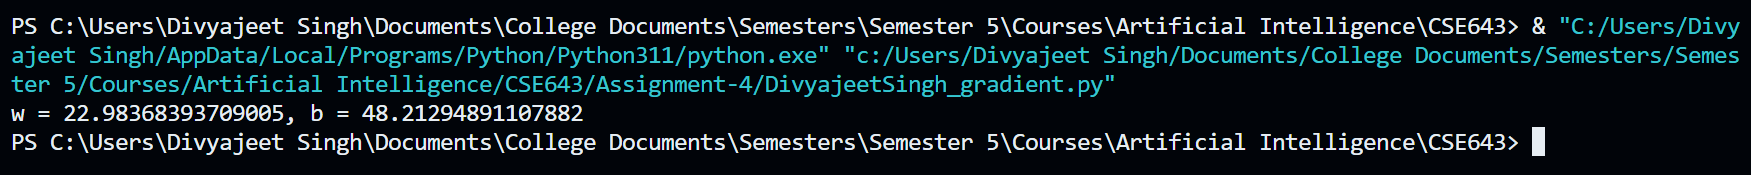
\includegraphics[width=\textwidth]{Assets/Regression.png}
    \end{figure}

    \section*{Problem 2}
    In this section, we were required to perform linear regression on the given dataset
    from the UCI-ML repository. The target is to achieve a threshold $R^{2}$ score.

    \begin{enumerate}[label=(\alph*)]
        \item To handle the categorical features, we use one-hot encoding. The column \texttt{"Sex"}
        was one-hot encoded using the \texttt{pandas.get\_dummies()} function.
        \item As per the hint, a non-linear transformation was performed on the continuous features.
        The transformation used was the square function. The modified features were appended
        to the original dataset.
        \begin{equation}
            \texttt{new\_feature} \gets \texttt{feature}^{2}
        \end{equation}
        The transformed features were used to train a linear regressor from the \texttt{sklearn}
        library. This achieved an $R^{2}$ score of 0.57 on the full dataset.
        \item 70-15-15 Cross Validation was performed for 100 iterations. The mean and standard
        deviation of the $R^{2}$ scores were calculated, which were 0.56 and 0.04 respectively.
    \end{enumerate}
    The code for the same is given in the file \texttt{DivyajeetSingh\_linear\_regression.py}.
    The box plot for the $R^{2}$ scores is shown in the following figure.

    \begin{figure}[htbp]
        \centering
        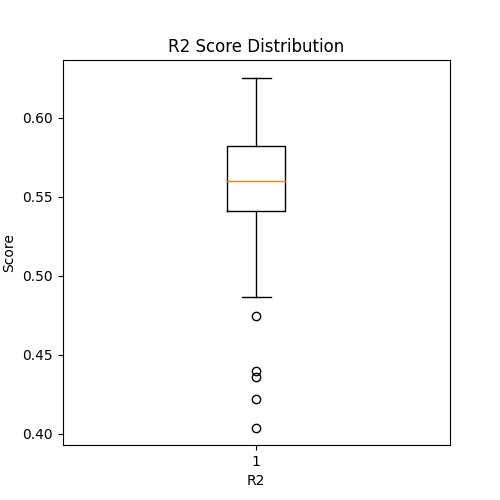
\includegraphics[width=\textwidth]{Assets/r2.png}
    \end{figure}

\end{document}